%-----------------------------------LICENSE------------------------------------%
%   This file is part of tikz_figures.                                         %
%                                                                              %
%   tikz_figures is free software: you can redistribute it and/or              %
%   modify it it under the terms of the GNU General Public License as          %
%   published by the Free Software Foundation, either version 3 of the         %
%   License, or (at your option) any later version.                            %
%                                                                              %
%   tikz_figures is distributed in the hope that it will be useful,            %
%   but WITHOUT ANY WARRANTY; without even the implied warranty of             %
%   MERCHANTABILITY or FITNESS FOR A PARTICULAR PURPOSE.  See the              %
%   GNU General Public License for more details.                               %
%                                                                              %
%   You should have received a copy of the GNU General Public License along    %
%   with tikz_figures.  If not, see <https://www.gnu.org/licenses/>.           %
%------------------------------------------------------------------------------%

% Use the standalone class for displaying the tikz image on a small PDF.
\documentclass[crop, tikz]{standalone}

% Import the tikz package to use for the drawing.
\usepackage{tikz}

% Package used for the LaTeX arrow.
\usetikzlibrary{arrows.meta}

% Begin the document.
\begin{document}

    % Begin the drawing.
    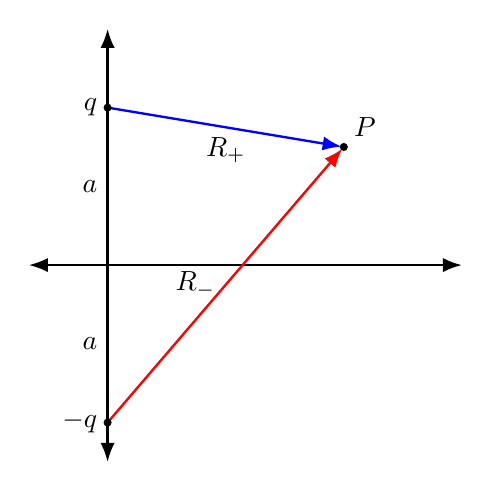
\begin{tikzpicture}[%
        line width = 0.3mm,
        > = Latex,
    ]

        % Position of the points.
        \coordinate (q) at (0.0, 2.0);
        \coordinate (-q) at (0.0, -2.0);
        \coordinate (P) at (3.0, 1.5);

        % Label the points.
        \node at (q) [left] {$q$};
        \node at (-q) [left] {$-q$};
        \node at (P) [above right] {$P$};

        % Draw coordinate axes.
        \draw[<->] (0.0, -2.5) to (0.0, 3.0);
        \draw[<->] (-1.0, 0.0) to (4.5, 0.0);

        % Draw lines from the points on the y axis to P.
        \begin{scope}[
            ->,
            shorten > = 0.8pt,
        ]
            \draw[draw = blue] (q) to node [below] {$R_{+}$} (P);
            \draw[draw = red] (-q) to node [left] {$R_{-}$} (P);
        \end{scope}

        % Mark the three points with dots.
        \filldraw (q) circle (1.0pt);
        \filldraw (-q) circle (1.0pt);
        \filldraw (P) circle (1.0pt);

        % Label the axes.
        \node at (0.0, 1.0) [left] {$a$};
        \node at (0.0, -1.0) [left] {$a$};
    \end{tikzpicture}
\end{document}
